\documentclass{article}
\usepackage[utf8]{inputenc}
\usepackage[greek,english]{babel}
\usepackage{alphabeta}
\usepackage{fancyhdr}
\usepackage{listings}
\usepackage{mathtools}
\usepackage{siunitx}
\usepackage{xcolor}
\usepackage{graphicx}
\usepackage{pgfplots}
\usepackage{tikz-timing}
\usepackage[export]{adjustbox}
\usepackage{biblatex}
\addbibresource{dl3-citations.bib}

%\pagestyle{fancy}
%\renewcommand\headrulewidth{0pt}
%\fancyhead{}
%\fancyfoot{}
%\fancyfoot[R]{\thepage}

\title{Εργαστηριακή Εργασία 3 - Flip-Flop}
\author{Χρήστος Μαργιώλης - 19390133 \\ Τμήμα 8}
\date{Ιούνιος 2020}

\begin{document}

\begin{figure}[t!]
    \centering
    
\includegraphics[scale=0.3, center]{./res/Logo_University_of_West_Attica.png}
    \Large
    \textbf{Πανεπιστήμιο Δυτικής Αττικής} \\
    \large
    Τμήμα Μηχανικών Πληροφορικής και Ηλεκτρονικών Υπολογιστών \\
    Ψηφιακή Σχεδίαση
\end{figure}
\begin{figure}[b]
    \centering
    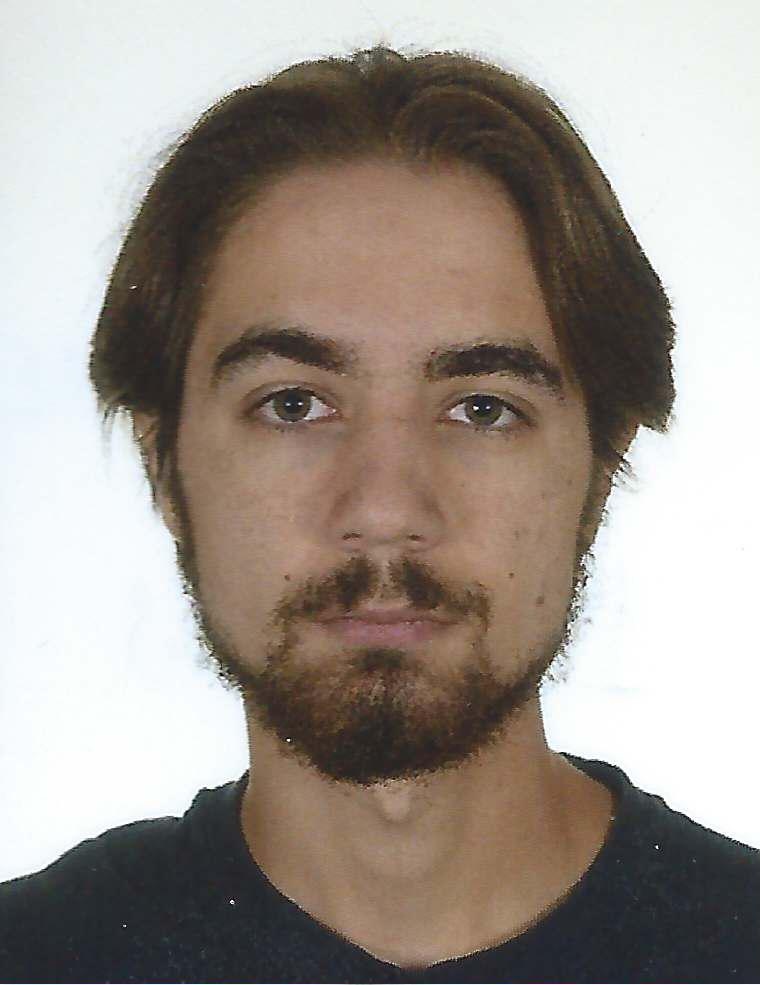
\includegraphics[scale=1]{./res/19390133.jpeg}
\end{figure}

\begin{titlepage}
\maketitle
\end{titlepage}

\renewcommand{\contentsname}{Περιεχόμενα}
\tableofcontents

\renewcommand{\abstractname}{Εισαγωγή}
\begin{abstract}
	Το αντικείμενο της εργασίας αυτής είναι η κατανόηση των μανδαλωτών
	και των Flip-Flop, μέσω θεωρητικών ασκήσεων και εφαμορμογών.
\end{abstract}
\pagebreak

\section{Συλλογή βιβλιογραφίας}
Η βιβλιογραφία που χρησιμοποιήθηκε κάλυψε τα βασικά προβλήματα
της εργασίας. Από την βιβλιογραφία πήρα πληροφορίες για την συμπεριφορά 
και την λειτουργία των διαφόρων ειδών μανδαλωτών και των Flip-Flop.

\section{Περιγραφή υλοποίησης}
Για την υλοποίηση της εργασίας και βασισμένος στην παραπάνω βιβλιογραφία
που συλλέχθηκε, χρησιμοποίησα κυκλώματα φτιαγμένα από λογικές πύλες, καθώς
και πίνακες αλήθειας για την απόδειξη και επαλήθευση των αποτελεσματών
που προέκυψαν από πειραματικές μετρήσεις.

\section{Εργαστηριακό μέρος}
\subsection{Μανδαλωτής με πύλες NAND}
Από την εφαρμογή του παρακάτω κυκλώματος παρατηρούμε ότι
ο πίνακας αλήθειας που προκύπτει πειραματικά πράγματι
επαληθεύει τον πίνακα αλήθειας του μανδαλωτή με πύλες NAND.

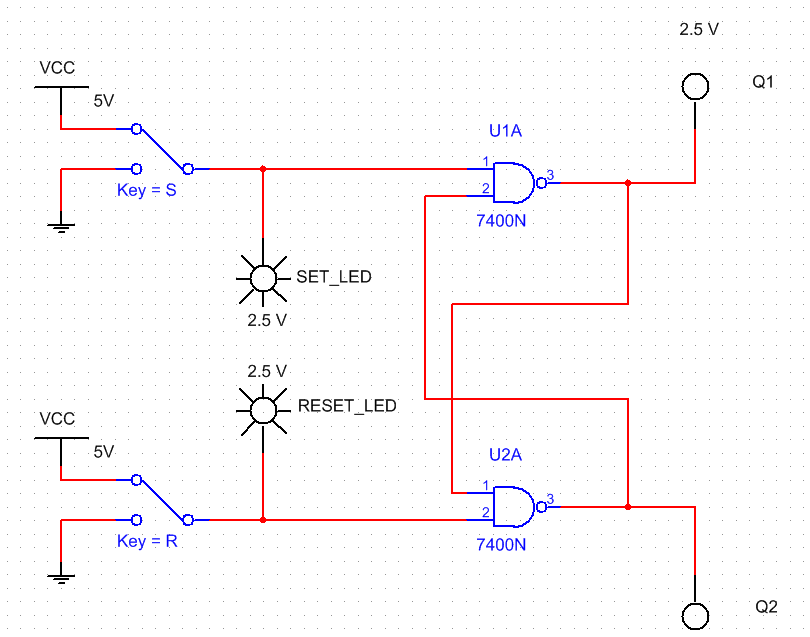
\includegraphics[width=\textwidth]{./res/ffnand.png}

\begin{center}
\begin{tabular}{|c|c|c|c|}
	\hline
	$S$ & $R$ & $Q_1$ & $Q_2$ \\
	\hline
	1 & 1 & $Q_1$ & $Q_2$ \\
	0 & 1 & 1 & 0 \\
	1 & 0 & 0 & 1 \\
	0 & 0 & 1 & 1 \\
	\hline
\end{tabular}
\end{center}

\subsection{R-S Flip-Flop}
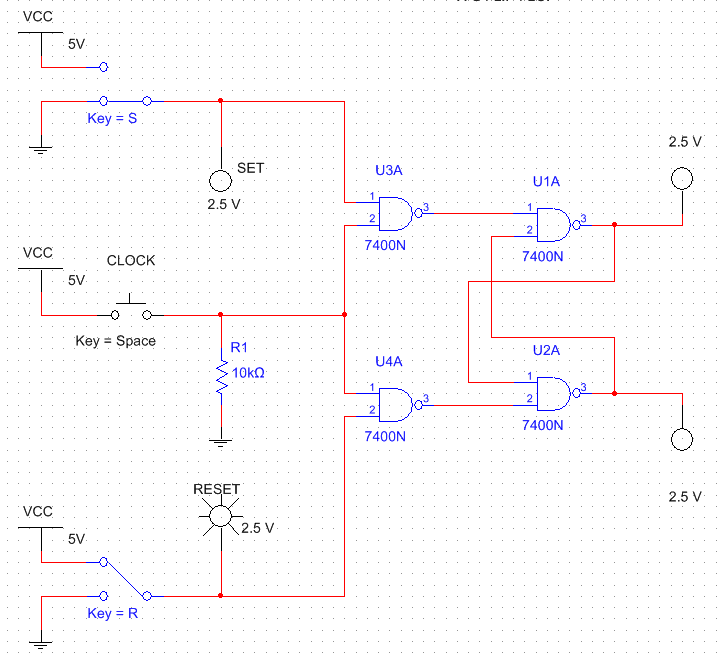
\includegraphics[width=\textwidth]{./res/rsff.png}

\begin{center}
\begin{tabular}{|c|c|c|}
	\hline
	$S$ & $R$ & $Q_{1(n+1)}$ \\
	\hline
	0 & 0 & $Q_1$ \\
	0 & 1 & 0 \\
	1 & 0 & 1 \\
	1 & 1 & $X$ \\
	\hline
\end{tabular}
\end{center}

\subsection{D Flip-Flop}
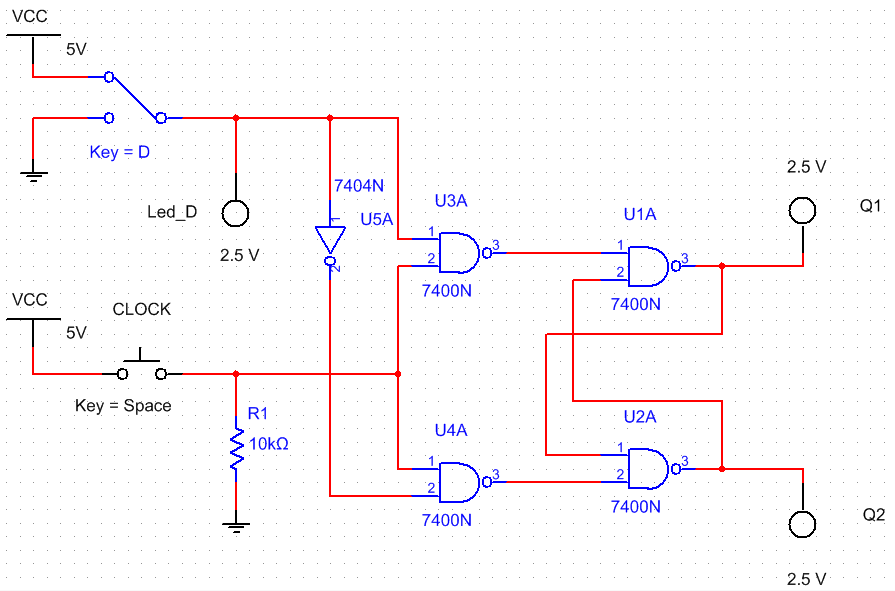
\includegraphics[width=\textwidth]{./res/dff.png}

\begin{center}
\begin{tabular}{|c|c|}
	\hline
	$D$ & $Q_{1(n+1)}$ \\
	\hline
	0 & 0 \\
	1 & 1 \\
	\hline
\end{tabular}
\end{center}

\subsection{J-K Flip-Flop}
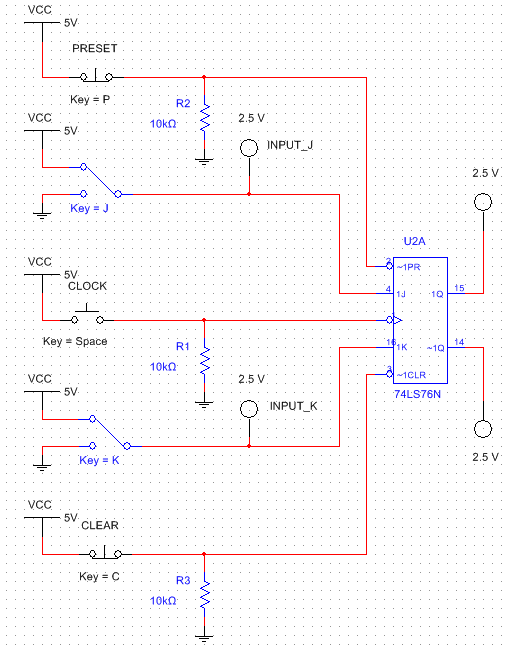
\includegraphics[width=\textwidth]{./res/jkff.png}

\begin{center}
\begin{tabular}{|c|c|c|}
	\hline
	$J$ & $K$ & $Q_{1(n+1)}$ \\
	\hline
	0 & 0 & $Q_{1n}$ \\
	0 & 1 & 0 \\
	1 & 0 & 1 \\
	1 & 1 & $Q_{1(n)}$ \\
	\hline
\end{tabular}
\end{center}

\subsection{Ερωτήσεις}
\begin{itemize}
	\item \textit{Γιατί πιστεύετε ότι χρειάζονται τα σύγχρονα ακολουθιακά κυκλώματα;} \\

	Τα σύχρονα ακολουθιακά κυκλώματα χρειάζονται επειδή σε αντίθεση με τα ασύγχρονα
	ακολουθιακά κυκλώματα, τα οποία ως κύρια στοιχεία μνήμης έχουν λογικές πύλες, έχουν
	flip-flops ως στοιχεία μνήμης. Αυτό σημαίνει ότι το flip-flop μπορεί να διατηρήση μια
	κατάσταση μέχρι κάποιο άλλο σήμα εισόδου να την αλλάξει. \cite{efstathiou} \\

	\item \textit{Πότε εμφανίζεται η επόμενη κατάσταση σε ένα Flip-Flop;} \\
	
	Η επόμενη κατάσταση σε ένα Flip-Flop εμφανίζεται όταν και οι δύο του είσοδοι
	$S$ και $R$ αντίστοιχα, είναι ίσες με λογικό 0. \\

	\item \textit{Ποιά η διαφορά του μανδαλωτή S-R και του S-R Flip-Flop;} \\

	Η διαφορά του μανδαλωτή S-R (S-R Latch) και του S-R Flip-Flop είναι ότι σε
	αντίθεση με το S-R Flip-Flop, ο μανδαλωτής S-R είναι πολύ ευαίσθητος στους
	ανεπιθύμητους παλμούς μικρού εύρους που μπορεί να εμφανιστούν στις εισόδους
	$S$ και $R$ \cite{efstathiou}.
	Επίσης ο μανδαλωτής S-R είναι ασύγχρονος, δηλαδή αλλάζει τιμή της εξόδου
	όταν αλλάζει η είσοδός του, ενώ το S-R Flip-Flop αλλάζει τιμή στην έξοδό του
	όταν το $CLK$ παίρνει τιμή λογικού 1. \\

	\item \textit{Από πού προκύπτει η ονομασία του D Flip-Flop} \\

	Η ονομοασία του D Flip-Flop προκύπτει από την λέξη Data Flip-Flop. Ο λόγος που έχει
	ονομαστέι έτσι είναι επειδή μπορεί να αποθηκεύει δεδομένα και να καθυστερεί την
	διάδοσή τους. \\

	\item \textit{Σχεδιάστε ένα T Flip-Flop με βάση το J-K Flip-Flop. Γράψτε το
		χαρακτηριστικό πίνακα λειτουργίας του.} \\

	\begin{center}
	\begin{tabular}{|c|c|c|}
		\hline
		$J$ & $K$ & $Q$	\\
		\hline
		0 & 0 & Q \\
		0 & 1 & 0 \\
		1 & 0 & 1 \\
		1 & 1 & $\overline{Q}$ \\
		\hline
	\end{tabular}
	\end{center}

	\item \textit{Ποιά είναι η συνθήκη για σωστή λειτουργία των Flip-Flop, και
			για ποιό λόγο σχεδιάστηκαν τα Master-Slave Flip-Flop;} \\

	Η συνθήκη που πρέπει να ισχύει για την σωστή λειτουργία των Flip-Flop είναι
	\[t_{on} < t_{pd} < T\]
	Τα Master-Slave Flip-Flop δημιουργήθηκαν επειδή δεν είναι πάντα εύκολο να
	ικανοποιηθεί αυτή η συνθήκη, διότι ο χρόνος $t_{pd}$ είναι πολύ μικρός, οπότε 
	τα Flip-Flop αυτού του τύπου λειτουργούν με βάση τους ορολογιακούς παλμούς. \\

	\item \textit{Τα καταωτέρω D Flip-Flop (σχήμα 20) έχουν αρχικές
			καταστάσεις $Q_0 = Q_1 = 0$. Δώστε σε χρονική αντιστοιχία 
			με το clock τις εξόδους $Q_0$ και $Q_1$ μέχρι να φαίνεται ένας
			πλήρης κύκλος λειτουργίας του κυκλώματος.} \\

	\begin{tikztimingtable}
		$CLK$ & 4L 8C 4C \\
		$Q_0$ & 16L \\
		$Q_1$ & 12L 4C \\
	\end{tikztimingtable}

	$Q_0 = Q_1 = 0$ \\
	$CLK = 0$ δεν αλλάζει \\
	$CLK = 1$ αν $D = 0$ τότε $Q = 0$, αν $D = 1$ τότε $Q = 1$ \\

	\begin{center}
	\begin{tabular}{|c|c|}
		\hline
		$D$ & $Q$ \\
		\hline
		0 & 0 \\
		1 & 1 \\
		\hline
	\end{tabular}
	\end{center}

	$CLK = 1$, $D_1 = \overline{Q_0} = Q_1 = D_0$

\end{itemize}

\renewcommand\refname{Πηγές}
\printbibliography
\end{document}
